\documentclass[border=10pt]{standalone}

\usepackage{tikz}
\usetikzlibrary{arrows.meta,arrows,decorations.pathmorphing,backgrounds,positioning,fit,petri,calc,shapes.geometric,scopes,fit,spy}
\usepackage{pgfplots}
\pgfplotsset{,compat=1.11}
\tikzset{/pgf/number format/1000 sep={\,}}

\usepackage{fontawesome5}
\renewcommand{\familydefault}{\sfdefault}
\usepackage{helvet}
\begin{document}

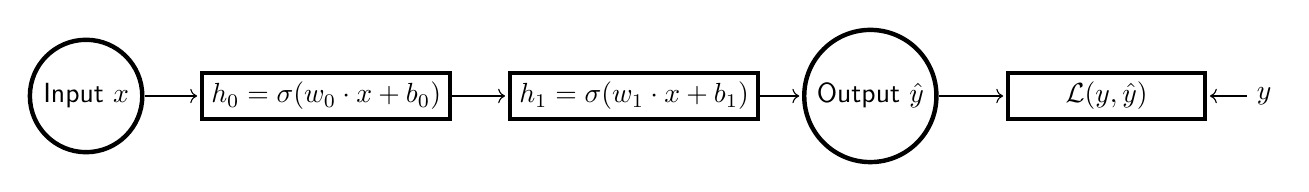
\begin{tikzpicture}[shorten >=1pt,node distance=3cm,auto]
   
   \node[ultra thick, draw, circle] (input) {Input $x$};
   \node[ultra thick, draw, rectangle] (hidden1) [right=2em of input] {$h_0=\sigma(w_{0} \cdot x + b_{0})$};
   \node[ultra thick, draw, rectangle] (hidden2) [right=2em of hidden1] {$h_1=\sigma(w_{1} \cdot x + b_{1})$};
   \node[ultra thick, draw, circle] (output) [right of=hidden2] {Output $\hat{y}$};
   \node[ultra thick, draw, rectangle, minimum width=2.5cm] (loss) [right of=output] {$\mathcal{L}(y, \hat{y})$};

   \path[->] (input) edge (hidden1)
   (hidden1) edge (hidden2)
   (hidden2) edge (output)
   (output) edge (loss);

   \node (ytrue) [right of=loss, node distance=2cm] {$y$};
   \path[->] (ytrue) edge (loss);
   
 \end{tikzpicture}
\end{document}
